\documentclass[12pt]{article}
\usepackage{graphicx}
\usepackage{float}
\usepackage{amsmath}
\begin{document}
\title{Electrical Engineering 113, Homework 5}
\date{May 15th, 2019}
\author{Michael Wu\\UID: 404751542}
\maketitle

\section*{Problem 1}

\paragraph{a)}

Since \(x[n]\) is a signal that is equal to \(1\) for \(n=0,\ldots,9\) and zero everywhere else,
we know that \(x[n]\) can be rewritten as the following expression.
\[x[n]=\sum_{m=0}^9 \delta(n-m)\]
Then since the DTFT of \(\delta(n)\) is \(1\), we can apply this along with linearity and the time
shifting property to obtain the following DTFT.
\[X(\Omega)=\sum_{m=0}^9 e^{-j\Omega m}\]
For \(h[n]\) we can apply the DTFT for signals of the form \(a^nu[n]\) to obtain the following result.
\[H(\Omega)=\frac{1}{1-0.8e^{-j\Omega}}\]

\paragraph{b)}

Using the convolution property we obtain the following result.
\[Y(\Omega)=\frac{\sum_{m=0}^9 e^{-j\Omega m}}{1-0.8e^{-j\Omega}}\]

\paragraph{c)}

First we perform the convolution to obtain the following result.
\[y[n]=\sum_{m=0}^9 (0.8)^{n-m}u[n-m]\]
Then we can apply the DTFT analysis equation as follows.
\begin{align*}
    Y(\Omega)&=\sum_{n=-\infty}^\infty \sum_{m=0}^9 (0.8)^{n-m}u[n-m] e^{-j\Omega n}\\
    &=\sum_{m=0}^9 \sum_{n=m}^\infty (0.8)^{n-m} e^{-j\Omega n}\\
    &=\sum_{m=0}^9 \sum_{n=0}^\infty (0.8)^{n} e^{-j\Omega (n+m)}\\
    &=\sum_{m=0}^9 \sum_{n=0}^\infty \left(0.8e^{-j\Omega}\right)^n e^{-j\Omega m}\\
    &=\sum_{m=0}^9 \frac{1}{1-0.8e^{-j\Omega}} e^{-j\Omega m}\\
    &=\frac{\sum_{m=0}^9 e^{-j\Omega m}}{1-0.8e^{-j\Omega}}
\end{align*}

\section*{Problem 2}

Begin with the DTFT of \(a^{2n}u[n]\). If we apply differentiation in frequency we can obtain the DTFT for \(na^{2n}u[n]\),
which is the same as the DTFT for \(na^{2n}u[n-1]=nx[n]\) since at \(n=0\) they are both equal to zero. Similarly we can
obtain the DTFT for \(n^2x[n]\) with the same property.
\begin{align*}
    j\frac{d}{d\Omega}\frac{1}{1-a^2e^{-j\Omega}}&=j\frac{-1}{(1-a^2e^{-j\Omega})^2}(ja^2e^{-j\Omega})\\
    &=\frac{a^2e^{-j\Omega}}{(1-a^2e^{-j\Omega})^2}
\end{align*}
\begin{align*}
    j\frac{d}{d\Omega}\frac{a^2e^{-j\Omega}}{(1-a^2e^{-j\Omega})^2}&=j\frac{-ja^2e^{-j\Omega}(1-a^2e^{-j\Omega})^2 - a^2e^{-j\Omega}2(1-a^2e^{-j\Omega})ja^2e^{-j\Omega}}{(1-a^2e^{-j\Omega})^4}\\
    &=j\frac{-ja^2e^{-j\Omega}(1-a^2e^{-j\Omega}) - a^2e^{-j\Omega}2ja^2e^{-j\Omega}}{(1-a^2e^{-j\Omega})^3}\\
    &=j\frac{-ja^2e^{-j\Omega}((1-a^2e^{-j\Omega}) + 2a^2e^{-j\Omega})}{(1-a^2e^{-j\Omega})^3}\\
    &=\frac{a^2e^{-j\Omega}(1+a^2e^{-j\Omega})}{(1-a^2e^{-j\Omega})^3}\\
\end{align*}
From the definition of the DTFT we can note that the sums \(\sum_{n=0}^\infty n^2x[n]\) and \(\sum_{n=0}^\infty nx[n]\)
are simply these expressions evaluated at \(\Omega=0\). Then we obtain the following result.
\begin{align*}
    \sum_{n=0}^\infty n^2x[n]&=\left.\frac{a^2e^{-j\Omega}(1+a^2e^{-j\Omega})}{(1-a^2e^{-j\Omega})^3}\right|_{\Omega=0}\\
    &=\frac{a^2(1+a^2)}{(1-a^2)^3}\\
    \sum_{n=0}^\infty nx[n]&=\left.\frac{a^2e^{-j\Omega}}{(1-a^2e^{-j\Omega})^2}\right|_{\Omega=0}\\
    &=\frac{a^2}{(1-a^2)^2}\\
    \frac{\sum_{n=0}^\infty n^2x[n]}{\sum_{n=0}^\infty nx[n]}&=\frac{1+a^2}{1-a^2}
\end{align*}

\section*{Problem 3}

\paragraph{a)}

\[X(\Omega)=e^{j\Omega 2} - 1 + e^{-j\Omega 2}\]

\paragraph{b)}

\[X[k]=e^{j\frac{2\pi k}{6} 2} - 1 + e^{-j\frac{2\pi k}{6} 2}\]

\paragraph{c)}

We only need to consider the portions of \(\tilde{x}[n]\) where \(0\leq n \leq 6\). Then we can use the following signal.
\[x[n] = -\delta[n] + \delta[n-2] + \delta[n-4]\]
We then obtain the following DTFS coefficients.
\begin{align*}
    c_k&=\frac{1}{6}\sum_{n=0}^5 x[n] e^{-j\frac{2\pi k}{6} n}\\
    6c_k&=-1 + e^{-j\frac{2\pi k}{6} 2} + e^{-j\frac{2\pi k}{6} 4}\\
    6c_k&=e^{j\frac{2\pi k}{6} 2} - 1 + e^{-j\frac{2\pi k}{6} 2} \\
    6c_k&=X[k]
\end{align*}

\section*{Problem 4}

The DFT of \(X[k]\) is equal to \(\sum_{k=0}^{N-1} X[k]e^{-j\frac{2\pi k}{N}n}\). From the
synthesis equation we also obtain the following result.
\begin{align*}
    x[n]&=\frac{1}{N}\sum_{k=0}^{N-1} X[k]e^{j\frac{2\pi k}{N}n}\\
    Nx[n]&=\sum_{k=0}^{N-1} X[k]e^{j\frac{2\pi k}{N}n}\\
    Nx[-n]&=\sum_{k=0}^{N-1} X[k]e^{-j\frac{2\pi k}{N}n}
\end{align*}
So \(y[n]\) is \(x[n]\) multiplied by a factor of \(N\) and going in the opposite direction.
Note that since we restrict \(n\) to be within \(0,\ldots, N-1\), it is not exactly \(y[n]=Nx[-n]\).
But since we apply this twice, the direction of \(w[n]\) is flipped once more and we obtain the
following result.
\[w[n]=N^2x[n]\]

\pagebreak

\section*{Problem 5}

\paragraph{a)}

I ran the following code.
\begin{verbatim}
fs = 100;
t = 0:1/fs:50;
x = 2*sin(2*pi*30*t)+3*sin(2*pi*20*(t-2))+3*sin(2*pi*10*(t-4));
N = length(x);
omega = 2*pi*(0:N-1)/N;
omega = fftshift(omega);
omega = unwrap(omega - 2*pi);
X = fft(x, N);
X = X/max(X);
set(gcf,'color','w');
plot(omega, abs(fftshift(X)), 'LineWidth', 2);
title('DTFT of x[n]', 'fontsize', 14);
set(gca, 'fontsize', 14);
xlabel('Radians', 'fontsize', 14);
export_fig problem5a.pdf;
\end{verbatim}
This produced the following output.
\begin{figure}[H]
    \begin{center}
        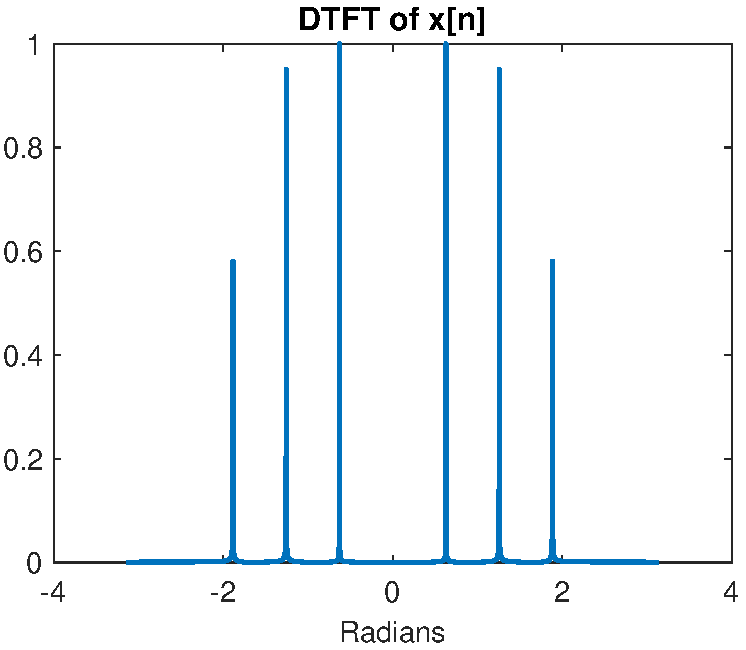
\includegraphics[width=3.5in]{problem5a.pdf}
    \end{center}
\end{figure}

\paragraph{b)}

I ran the following code.
\begin{verbatim}
wr = t<=2;
Xr = fft(x.*wr, N);
Xr = Xr/max(Xr);
plot(omega, abs(fftshift(Xr)), 'LineWidth', 2);
title('DTFT of x[n]w_r[n]', 'fontsize', 14);
set(gca, 'fontsize', 14);
xlabel('Radians', 'fontsize', 14);
export_fig problem5b.pdf;
\end{verbatim}
This produced the following output.
\begin{figure}[H]
    \begin{center}
        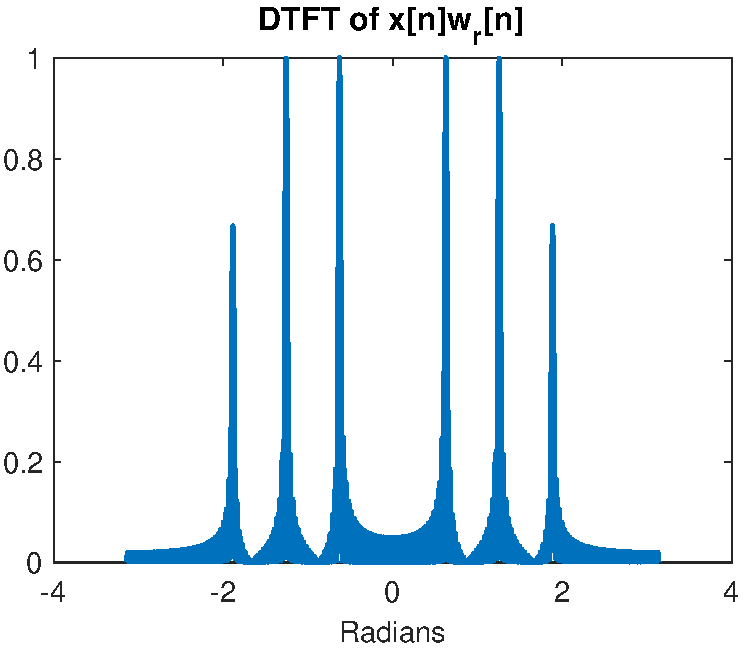
\includegraphics[width=3.5in]{problem5b.pdf}
    \end{center}
\end{figure}

\paragraph{c)}

I ran the following code.
\begin{verbatim}
wh = hamming(2*fs + 1).';
wh(N) = 0;
Xh = fft(x.*wh, N);
Xh = Xh/max(Xh);
plot(omega, abs(fftshift(Xh)), 'LineWidth', 2);
title('DTFT of x[n]w_h[n]', 'fontsize', 14);
set(gca, 'fontsize', 14);
xlabel('Radians', 'fontsize', 14);
export_fig problem5c.pdf;
\end{verbatim}
This produced the following output.
\begin{figure}[H]
    \begin{center}
        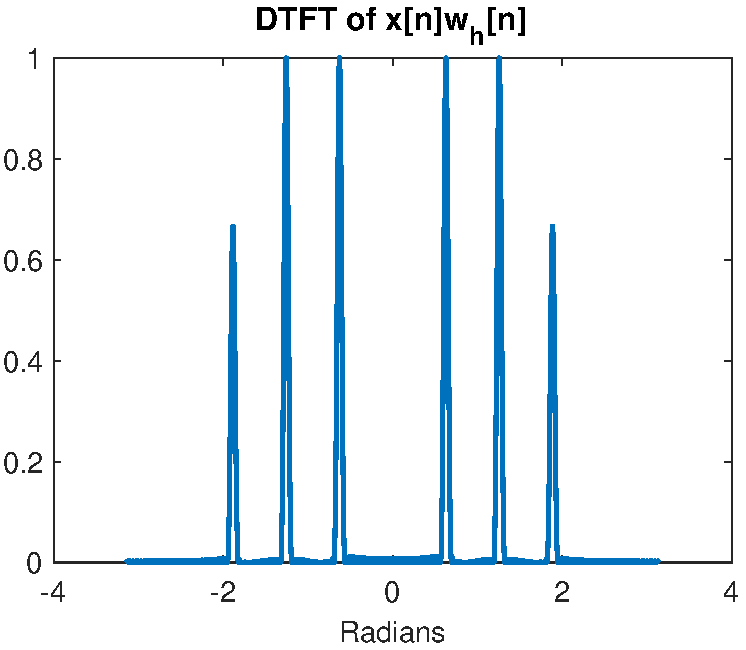
\includegraphics[width=3.5in]{problem5c.pdf}
    \end{center}
\end{figure}

\paragraph{d)}

The original signal has sharply defined peaks around the following values.
\[\Omega=\pm0.2\pi, \pm0.4\pi, \pm0.6\pi\]
These peaks correspond to the three sinusoids. The peaks at \(\pm0.6\pi\) are smaller than the other peaks since
the corresponding component has a coefficient of \(2\) while the other components have a coefficient of \(3\). We see
that rectangular windowing produces similar peaks, but there are more surrounding frequency components in the frequency spectrum
around the main peaks. The result is that the frequency spectrum appears more noisy and less well defined than the graph of the
original signal. With the Hamming window, we are able to recover the original peaks while reducing any extra frequency components.
The heights of the peaks also correspond to the correct magnitude ratios, as the peaks at \(\pm0.6\pi\) have a magnitude of
approximately \(\frac{2}{3}\). The other peaks have magnitude \(1\). This is beneficial since we can see the intended frequency
spectrum while reducing storage size by 25 times.

\end{document}